\documentclass[a4paper, 12pt]{report}
\usepackage[ngerman]{babel}
\usepackage{amssymb}
\usepackage{amsmath}
\usepackage{bbm}
\usepackage{graphicx}
\usepackage[style=alphabetic ,backend=biber]{biblatex}
\usepackage{csquotes}
\addbibresource{../Facharbeit/literatur.bib}
\usepackage{listings}
\usepackage{xcolor}

\definecolor{codegreen}{rgb}{0,0.6,0}
\definecolor{codegray}{rgb}{0.5,0.5,0.5}
\definecolor{codepurple}{rgb}{0.58,0,0.82}
\definecolor{backcolour}{rgb}{255,255,255}

\lstdefinestyle{codehighligthing}{
    backgroundcolor=\color{backcolour},
    commentstyle=\color{codegreen},
    keywordstyle=\color{magenta},
    numberstyle=\tiny\color{codegray},
    stringstyle=\color{codepurple},
    basicstyle=\ttfamily\footnotesize,
    breakatwhitespace=false,
    breaklines=true,
    captionpos=b,
    keepspaces=true,
    numbers=left,
    numbersep=5pt,
    showspaces=false,
    showstringspaces=false,
    showtabs=false,
    tabsize=2
}
\lstset{style=codehighligthing}

\title{Facharbeit Informatik}
\author{Joel Mantik}
\begin{document}
\maketitle
\begin{sloppypar}
\tableofcontents

\chapter{Einleitung}
\begin{quote}
    "The simplest model in applied mathematics is a system of linear equations. It is also by far the most important."
    \newline GILBERT STRANG
\end{quote}
Der Gauß-Algorithmus ist eins der wichtigsten Lösungsverfahren zum Lösen lineare
r Gleichungssysteme.
Er spielt eine tragende Rolle in vielen Bereichen der Mathematik und ist dennoch  recht unkompliziert.
    Aufgrund der Wichtigkeit, habe ich dazu entschieden, den Algorithmus in dieser
Facharbeit zu implementieren,
zu analysieren, und Anwendungsmöglichkeiten aufzuzeigen.

\chapter{Theoretische Grundlagen}
Der Gauß-Algorithmus ist ein Algorithmus, welcher beim Lösen von linearen Gleichungssystemen zum Einsatz kommt. Im folgenden Kapitel wird die mathematische Theorie
von linearen Gleichungssystemen und dem Gauß-Algorithmus erläutert, welche die Grundlage für die spätere Implementierung sind.
Die folgenden Definitionen sind sinngemäß aus \cite{gramlich2021} entnommen.
\section{Lineare Gleichungssysteme}
Ein lineares Gleichungssystem ist eine Sammlung von Gleichungen, in denen jede Unbekannte mit höchstens dem ersten Grad vorkommt.
Es kann in der Form $ A_x = b $ geschrieben werden, wobei $A$ eine $ m * n $ Matrix ist, $x$ ein n-dimensionaler Vektor von Unbekannten
und b ein $m$-dimensionaler Vektor von Konstanten ist.
Ein allgemeines lineares Gleichungssystem lässt sich wie folgt definieren. :
\begin{align*}
    a_{11}x_{1}+ a_{12}x_{2}+\hdots+ a_{1n}x_{n} = b_1 \\
    a_{21}x_{1}+ a_{22}x_{2}+\hdots+ a_{2n}x_{n} = b_2\\
    a_{11}x_{1}+ a_{12}x_{2}+\hdots+ a_{1n}x_{n} = b_3 \\
    \vdots \\
a_{m1}x_{1}+ a_{m2}x_2+\hdots+a_{mn}x_{n} = b_{m}
\end{align*}
\newpage
Das Ziel eines solchen linearen Gleichungssystems ist es, eine Lösung für $x$ zu finden, die alle Gleichungen erfüllt.
Hierbei gibt es drei Arten von Lösungen:
\begin{enumerate}
    \item Das Gleichungssystem hat genau \textit{eine} Lösung; es gibt genau eine Lösung, welche alle Gleichungen im System erfüllt. Die Lösungsmenge ist z. B. : $\mathbb{L} = \{ (x,y,z)| (1,2,3)\} $.
    \item Das Gleichungssystem hat \textit{keine} Lösung, wenn es keine Lösung gibt, die alle Gleichungen erfüllt. Die Lösungsmenge ist eine leere Menge: $\mathbb{L} = \{ \}$.
    \item Das Gleichungssystem hat \textit{unendlich viele} Lösungen, wenn es mehrere Lösungen gibt, die alle Gleichungen im System erfüllen.
        Hierbei sind die verschiedenen Variablen voneinander abhängig. Die Lösungsmenge sieht beispielsweise wie folgt aus: \newline $ \mathbb{L} = \{(x, y, z)| (x = y * z, y\in \mathbb{R}, z \in \mathbb{R}) \} $.
\end{enumerate}


\section{Gaußsches Eliminationsverfahren}
\chapter{Implementierung des Algorithmus}
Für die im Folgenden dargelegte Implementation und Analyse des Algorithmus wurde die Programmiersprache "Java" verwendet.
\section{Schritte des Verfahrens}
Grundlegend lässt sich der Algorithmus durch folgende Schritte implementieren, es gibt bei gewissen Implementationen (wie der Brute-Force Methode)
zwar kleine Abweichungen jedoch folgen auch diesen demselben Prinzip.
\begin{enumerate}
    \item Eingabe: Ein lineares Gleichungssystem $ A_x=b $ mit einer $ n * n $ Matrix $A$ und einem \textit{n}-dimensionalem Vektor b.
    \item Initialisierung: % weiter erläutern %
    \item Pivotisierung: Finden des größten Elements $a_{ki}$ in der Spalte von $A$ unterhalb der Diagonalen und tauschen der Zeilen $k$ und $i$ von $A$ und $B$.
    \item Elimination: %...%
    \item Rückwärtssubstitution: %...%
\end{enumerate}
Der Aufbau des Algorithmus wird in folgendem Diagramm deutlich:
\begin{figure}[h]
    \centering
    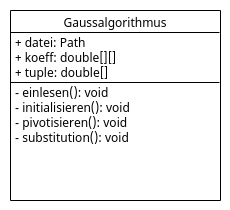
\includegraphics[width=150px]{"./gaussuml.png"}
    \caption{Implementationsdiagramm der Klasse Gauß-Algorithmus}
\end{figure} \newpage
\section{Erläuterung des Quellcodes}


\section{Beispielrechungen}
\section{Schwächen des Algorithmus}
\chapter{Anwendungen des Gaußschen-Eliminationsverfahrens}
\section{Lösung von linearen Gleichungssystemen}
\section{Inversion von Matrizen}
\section{Beispielanwendungen}
\chapter{Abwägungen}
\section{Vorteile im Vergleich zu anderen Methoden}
\section{Nachteile im Vergleich zu anderen Methoden}
\chapter{Fazit}
\chapter{Anhang}
\lstinputlisting[language=Java, caption=Quellcode des Gauß-Algorithmus]{./Quellcode/Gauss.java}
\printbibliography
\end{sloppypar}
\end{document}
